\documentclass[11pt,a4paper]{article}

\usepackage[T1]{fontenc}
\usepackage[utf8]{inputenc}
\usepackage{lmodern}
\usepackage[margin=2.4cm]{geometry}
\usepackage{booktabs}
\usepackage{graphicx}
\usepackage{amsmath}
\usepackage{caption}
\usepackage{enumitem}
\usepackage{xcolor}
\usepackage[hidelinks]{hyperref}
\usepackage{titlesec}

\definecolor{accent}{HTML}{1F4E79}
\captionsetup{font=small,labelfont=bf,labelsep=endash,skip=4pt}
\titleformat{\section}{\large\bfseries\color{accent}}{\thesection}{0.6em}{}
\titleformat{\subsection}{\normalsize\bfseries}{\thesubsection}{0.6em}{}
\setlength{\parskip}{0.35em}
\setlist{itemsep=2pt,topsep=2pt}

\newcommand{\code}[1]{\texttt{\small #1}}

\title{\textbf{From Post Text to User Network}\\[0.3em]
\large Generating a Temporal Social Network by Transferring tNodeEmbed}
\author{Angelantonio Fedele Murolo}
\date{}

\begin{document}
\maketitle

\begin{abstract}
\noindent
We reconstruct the link structure of a population for which only the text of its posts is observed: no
edges, no dates. The edge-formation mechanism is learned on a real social network of 25,714 users,
824,045 directed edges and nine snapshots, and applied by generation to a synthetic dataset of 10,000
users described only by their posts. The temporal model is tNodeEmbed without node2vec, initialised with
content representations. The generator is fitted on the real transitions and samples the network step by
step through arrival events, so the unit is the entering user rather than the pair. Two synthetic
networks come from the same pipeline and two temporal partitions, named after the partition they come
from. The \emph{progressive} network, in which users enter over time, is the one we present; the
\emph{all-present} network, in which the whole population exists from the first step, is kept as a
comparison. The progressive network reproduces reciprocity (0.3224 against 0.4177), mean degree (27.45
against 32.05), maximum degree (274 against 1,290), transitivity (0.0212 against 0.0337), clustering
(0.042 against 0.080) and diameter (6 against 6) within the right order of magnitude. The content does
not decide who links to whom. The content term weighs $+0.05$ in the edge-formation model against
$+1.22$ for ``the counterpart is new'', and the 2.13 content homophily of the real network is largely
degree structure.
\end{abstract}

\tableofcontents
\newpage

\section{Business understanding}

\subsection{Business goals}
A social platform that holds only the text produced by its users, with no follow graph, no interaction
log and no reliable time stamp, cannot compute reach, communities or influence. All of these need the
network. Buying or scraping the graph is often impossible: the data are not public, the platform is
small, or the graph is precisely what the platform wants to hide. The business goal is therefore to
\emph{reconstruct} the missing link structure from the only asset available, the text, and to do so
without inventing statistics.

\subsection{Data mining goals}
Translated into measurable goals:
\begin{itemize}
  \item \textbf{G1}: learn, from a dataset that does have a network, the mechanism by which an edge is
        formed, and express it as a model whose coefficients can be read and discussed;
  \item \textbf{G2}: apply that mechanism to a second population, of different size and with no
        edges, generating a network that is statistically comparable to the first;
  \item \textbf{G3}: quantify how much the text contributes, separating what comes from content from
        what comes from structure;
  \item \textbf{G4}: declare and measure the assumptions that remain ours (the temporal scenario, the
        transfer across populations of different size, the non-reproducibility of training).
\end{itemize}
The deliverable is a reproducible pipeline plus the generated network, not a single number.

\section{Data understanding}

\subsection{Data collection}
Two datasets were provided for the project. The \emph{real} dataset contains users, their posts and the
directed links between them over nine cumulative snapshots from January 2022 to July 2025. The
\emph{synthetic} dataset contains 10,000 users with 100,456 usable posts, eleven profile attributes and
\emph{no} edges and \emph{no} dates. The real dataset carries only post-level fields: there is no profile
attribute on the real side. The two datasets were never modified; every generated folder is a new
artefact.

\subsection{Data description}
\begin{table}[h]
  \centering
  \small
  \caption{The two datasets.}
  \begin{tabular}{@{}lll@{}}
    \toprule
    & Real & Synthetic \\
    \midrule
    Users & 25,714 & 10,000 (9,913 with at least one post) \\
    Posts & 173,475 cumulative / 154,580 per period & 100,456 usable \\
    Edges (directed) & 824,045 & none \\
    Time & 9 snapshots, Jan 2022 to Jul 2025, split 6/1/2 & none: 4 native batches, random order \\
    Per user & post text only & 11 profile labels, post text \\
    Shared column & \code{content} & \code{content} \\
    \bottomrule
  \end{tabular}
\end{table}

The eleven labels of the synthetic side are listed in Table~\ref{tab:labels}. Nine of them are finite
classes; \code{username} and \code{user\_bio} are free text (and usernames are reused across users,
671 distinct strings for 9,913 users), and \code{interests} is a short list rather than a single class.
None of the eleven exists on the real side, so they are never used as inputs: they serve as prediction
targets in Section~\ref{sec:content}.

\begin{table}[h]
  \centering
  \small
  \caption{The eleven profile labels of the synthetic dataset, counted over the 9,913 users with at
  least one post.}
  \label{tab:labels}
  \begin{tabular}{@{}lrl@{}}
    \toprule
    Label & Distinct values & Note \\
    \midrule
    \code{nationality}          & 1     & all \emph{american} \\
    \code{gender}               & 2     & female, male \\
    \code{ethnicity}            & 4     & four classes \\
    \code{political\_leaning}   & 7     & seven classes, prediction target \\
    \code{age\_interval}        & 9     & nine bands, eight populated in the sample \\
    \code{religion}             & 12    & twelve classes \\
    \code{state\_of\_origin}    & 50    & the fifty US states \\
    \code{interests}            & 32    & list, mean 1.5 terms per user (max 3); 112 users empty \\
    \code{profession}           & 41    & forty-one classes, prediction target \\
    \code{username}             & 671   & free text, reused across users \\
    \code{user\_bio}            & 5,605 & free text, one sentence per user \\
    \bottomrule
  \end{tabular}
\end{table}

Two facts of the real network govern the design. First, \textbf{no new edge connects two users who were
already present}: the share of ``pre-existing to pre-existing'' edges is $0.0000\%$ in every transition,
so each edge can be attributed to the arrival of its new endpoint. Second, the network is extremely
unequal: mean out-degree $32.05$, median $4$, maximum $1{,}290$.

The synthetic dataset has no dates. The only available order is the dense post identifier, which we
assume reflects the generation order; the four native batches are \emph{not} periods (each covers the
whole identifier range and shares about 9,500 users with the others, and the fourth has two rows).

\section{Data preparation}

\subsection{Data selection}
Module \code{graph\_io.py} reads edges, posts and attributes; self-loops are dropped (one artefact in the
real data), identifiers are normalised. Snapshots are cumulative and ordered; a transition is the
difference between consecutive snapshots. The evaluation split is temporal: five transitions for
training, one for validation (2025-07-01/20), two for test (2025-07-21/28 and 2025-07-29/31), and the
test windows are not touched until evaluation.

\subsection{Features}
The only column present on both sides is the post text. Each post is encoded \emph{individually} and the
vectors of a user are averaged into one representation per user and snapshot. Six encoders were
compared with the full downstream protocol, using matched negatives as the deciding column
(Table~\ref{tab:encoders}).

\begin{table}[h]
  \centering
  \small
  \caption{Encoder selection on the real network: AUC on validation / test1 / test2, mean over the three
  windows, and random negatives on validation.}
  \label{tab:encoders}
  \begin{tabular}{@{}lccc@{}}
    \toprule
    Encoder & val / test1 / test2 & mean & random negatives (val) \\
    \midrule
    tf-idf + SVD            & 0.489 / 0.521 / 0.505 & 0.505 & 0.986 \\
    \textbf{all-MiniLM-L6-v2} & 0.571 / 0.521 / 0.510 & \textbf{0.534} & 0.995 \\
    BGE-small               & 0.541 / 0.517 / 0.519 & 0.526 & 0.996 \\
    GTE-small               & 0.529 / 0.514 / 0.507 & 0.516 & 0.996 \\
    BGE-base                & 0.540 / 0.517 / 0.535 & 0.530 & 0.996 \\
    GTE-base                & 0.543 / 0.523 / 0.531 & 0.532 & 0.996 \\
    \bottomrule
  \end{tabular}
\end{table}

Encoding per post improves every encoder over concatenating a user's posts into one string, which the
encoder truncated at its token limit (for the most active users only 28\% of tokens survived): the mean
rises from 0.534 to \textbf{0.549} for MiniLM, from 0.530 to 0.540 for BGE-base, from 0.505 to 0.524 for
tf-idf. \textbf{MiniLM with per-post encoding} is the representation used downstream.

The margin between the first and the third encoder (0.002) is \emph{within} the variability between
processes, which is about 0.005 because the iteration order of edge sets is not fixed in Python and
changes negative sampling. The selection should therefore be read as a tie among MiniLM, GTE-base and
BGE-base, all clearly above tf-idf. We declare that limitation rather than hide it.

\subsection{Integration: the temporal partition}
The synthetic dataset is partitioned into nine steps, equal to the number of real snapshots, with two
rules measured on the real data: the \textbf{arrival curve} (share of users entering at each step when
users are ordered by their first post: $0.418$, $0.142$, $0.110$, $0.072$, $0.078$, $0.051$, $0.010$,
$0.077$, $0.042$) and the \textbf{activity shape} (posts per active user per period sampled from the
real distribution: mean 3.7, median 2, p90 9, bursts placed at random). The aggregate posts-per-snapshot
curve of the real data is \emph{not} used: real snapshots have heterogeneous lengths, so those counts
measure activity times window length.

Two partitions are produced. In the \textbf{progressive-arrival} one users enter following the real
curve; in the \textbf{all-present} one every user exists from the first step and only the activity shape
is kept. Both contain the same population and the same text.

\section{Modeling}

\begin{figure}[h]
  \centering
  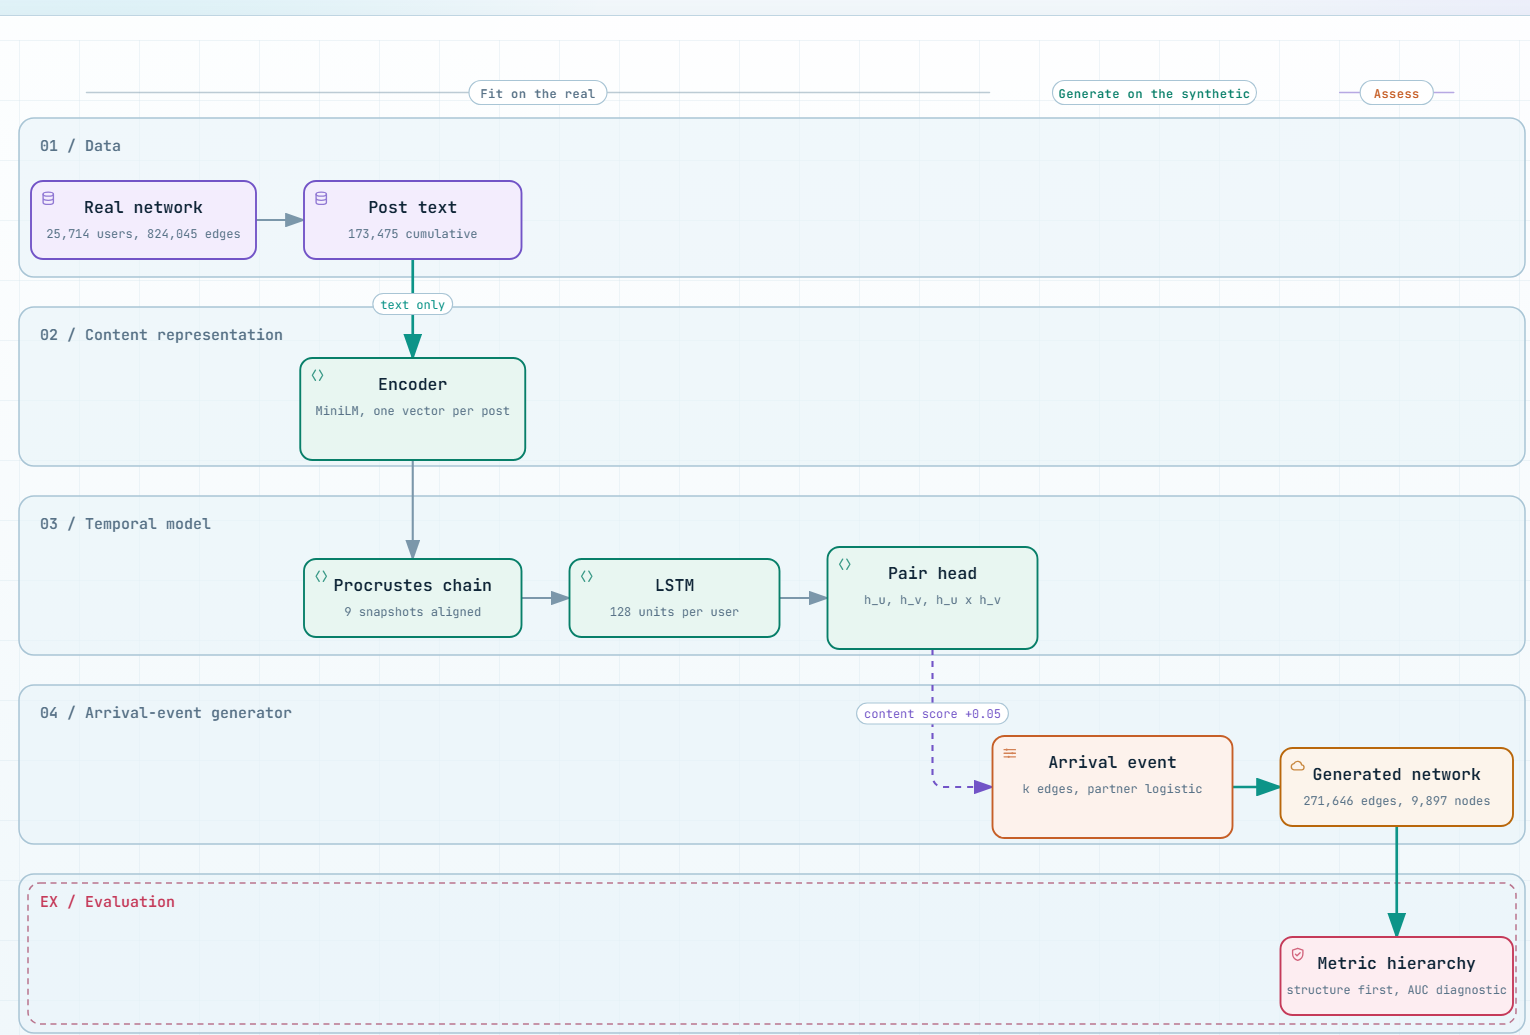
\includegraphics[width=\textwidth]{results/figures/pipeline_diagram.png}
  \caption{The pipeline. Post text is encoded per post, the nine snapshots are aligned and read by the
  LSTM, the pair head scores a candidate partner, and the generator samples arrival events on the
  synthetic population. Quantities in the boxes are those of the progressive network.}
  \label{fig:pipeline}
\end{figure}

\subsection{Evaluation protocol and metric hierarchy}
A generated network is not evaluated with an AUC: in the synthetic dataset there are no true edges to
predict, so a ranking measure has no object. The hierarchy we adopt is explicit.
\begin{itemize}
  \item \emph{Primary}: per-snapshot network statistics and distributions, compared with the real
        network on the final snapshot. These are the degree distribution (mean, maximum, CCDF),
        reciprocity, transitivity and mean clustering, modularity, diameter, composition of accretion.
  \item \emph{Secondary}: the nature of the link, that is content homophily with structural controls,
        and the share of edges between users arriving in the same step.
  \item \emph{Diagnostic, on the real data only}: AUC and average precision with matched and random
        negatives, used to select the encoder and to fit the model. The AUC ablation on the real data
        is saturated (0.9818 to 0.9816) and does not measure the contribution of text.
  \item \emph{Not valid}: AUC as a quality measure of a generated network.
\end{itemize}

\subsection{Architecture: tNodeEmbed without node2vec}
For each snapshot we hold a users~$\times$~dimension matrix from content. A \textbf{chain of orthogonal
Procrustes alignments} between consecutive snapshots brings the representations into a common coordinate
system; an \textbf{LSTM} (128 units) reads the sequence of the nine steps of each user; a \textbf{pairwise
head} on $[h_u, h_v, h_u \odot h_v]$ produces the link score. Training is binary cross-entropy on the
training transitions only.

Removing node2vec is a data-driven choice: node2vec initialises itself by observing links, so it cannot
represent a user appearing for the first time, and on this dataset no new edge connects two already
present users. Applying the original protocol restriction (test limited to pairs between already
observed users) yields \emph{zero} test edges in every transition. The restriction is correct in general
and empty here, so evaluation uses the whole transition with two kinds of negatives:
\emph{random} and \emph{matched} (same source, similar arrival snapshot and degree). Random negatives
give AUC around 0.99 in validation and 0.95--0.97 in test; matched negatives give 0.51--0.57. The matched
column is the one we report.

\subsection{Training}
Five transitions, twenty thousand positives and twenty thousand matched negatives per transition, eight
epochs, Adam at $10^{-3}$. The trained model (encoder, Procrustes, LSTM, head) is then frozen and applied
to the synthetic users: the encoder is the same, so the representation space is shared and no new
alignment is needed.

\subsection{The generator: arrival events}
The generator is fitted on the real transitions and estimates four things: how many edges an arrival
carries ($k$, from a table normalised on the population and rescaled at generation time), the direction
of each edge, the share of immediately reciprocated pairs (by direction and degree class), and the choice
of the counterpart, a logistic regression on seven standardised variables.

\begin{table}[h]
  \centering
  \small
  \caption{Coefficients of the counterpart-choice model, fitted on the real transitions.}
  \begin{tabular}{@{}lr@{\hspace{2em}}lr@{}}
    \toprule
    Variable & Coef. & Variable & Coef. \\
    \midrule
    Content score (pair head) & $+0.049$ & Partner active in the step & $-0.026$ \\
    $\log(1+\text{degree})$ & $+1.021$ & Direction (outgoing) & $+0.139$ \\
    Degree percentile & $+0.909$ & Co-occurrence in the event & $+0.194$ \\
    Counterpart is new & $+1.216$ & Validation AUC & $0.918$ \\
    \bottomrule
  \end{tabular}
\end{table}

Generation proceeds step by step. For each entering user, $k$ edges are drawn; for each edge the partner
is chosen with the fitted logistic on the \emph{current} state (degrees, percentiles, novelty, activity,
neighbourhood), plus Gumbel noise to sample rather than take the argmax. No threshold and no count is
imposed: volume, degrees and hubs emerge.

\subsection{Model assessment}
The real network is not modified. Structurally, the generator reproduces the shape of accretion (no
edge between two pre-existing users, as in the real data) while slightly overestimating edges between
co-arriving users (17.0\% against 8.1\%). The residual gaps are all of the same sign: the generated
network is somewhat flatter. The measurement attributes them to the shape of the tail and to cohesion,
not to a missing hub (Section~\ref{sec:eval}).

\section{Evaluation}
\label{sec:eval}

\subsection{The progressive network and the all-present comparison}
\begin{table}[h]
  \centering
  \small
  \caption{Last snapshot: real network, progressive network (users entering over time) and all-present
  network (comparison). Best value per row is not marked: the two synthetic networks are equivalent
  overall (Section~\ref{sec:part}).}
  \label{tab:main}
  \begin{tabular}{@{}lrrr@{}}
    \toprule
    & Real & Progressive & All-present \\
    \midrule
    Nodes with an edge      & 25,714 & 9,897 & 9,901 \\
    Edges                   & 824,045 & 271,646 & 280,298 \\
    Density                 & 0.00125 & 0.00277 & 0.00286 \\
    Mean out-degree         & 32.05 & 27.45 & 28.31 \\
    Maximum out-degree      & 1,290 & 274 & 328 \\
    Reciprocity             & 0.4177 & 0.3224 & 0.3035 \\
    Modularity              & 0.2751 & 0.1074 & 0.1030 \\
    Transitivity            & 0.0337 & 0.0212 & 0.0209 \\
    Mean clustering         & 0.0804 & 0.0420 & 0.0435 \\
    Content homophily       & 2.13 & 1.001 & 0.999 \\
    Diameter (approximate)  & 6 & 6 & 6 \\
    Out-degree tail slope   & $-2.349$ & $-3.980$ & $-3.332$ \\
    \bottomrule
  \end{tabular}
\end{table}

\begin{figure}[h]
  \centering
  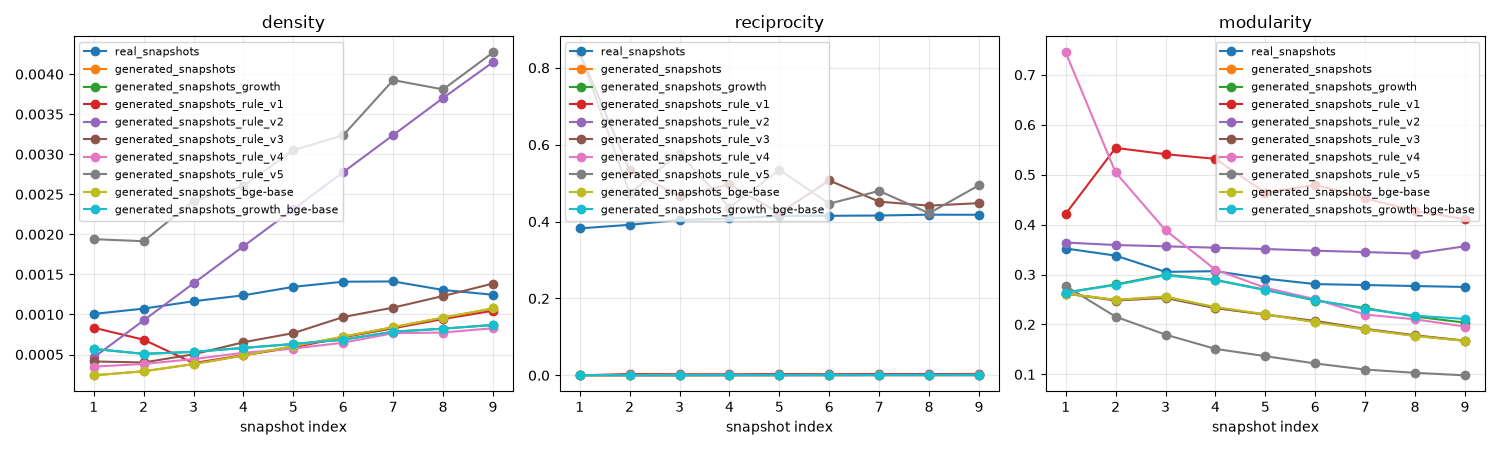
\includegraphics[width=\textwidth]{results/figures/compare_structure.png}
  \caption{Density, reciprocity and modularity per snapshot: real network, progressive network,
  all-present network.}
\end{figure}

How the new edges are composed says more than the totals. In the real network no edge joins two
pre-existing users; the progressive network reproduces that shape and slightly overestimates edges between
co-arriving users.

\begin{table}[h]
  \centering
  \small
  \caption{Composition of the new edges, pooled over the transitions, last snapshot.}
  \begin{tabular}{@{}lrr@{}}
    \toprule
    & Real & Progressive \\
    \midrule
    New to pre-existing            & 48.9\% & 45.2\% \\
    Pre-existing to new            & 43.0\% & 37.7\% \\
    New to new                     &  8.1\% & 17.0\% \\
    Pre-existing to pre-existing   &  0.0\% &  0.0\% \\
    Mean prior degree, existing end & 436.9 & 153.3 \\
    Mean prior degree, all nodes    &  64.4 &  51.5 \\
    \bottomrule
  \end{tabular}
\end{table}

\begin{figure}[h]
  \centering
  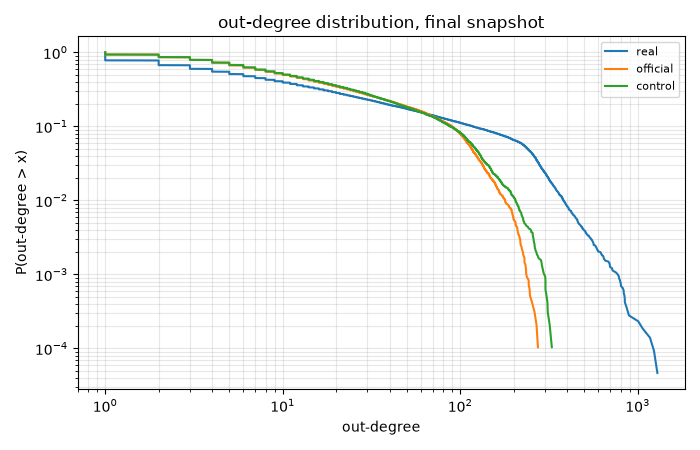
\includegraphics[width=0.78\textwidth]{results/figures/compare_degree_ccdf.png}
  \caption{Out-degree distribution (CCDF) at the last snapshot. At matched size the generated tail is
  steeper than the real one: the hubs are relatively less extreme.}
\end{figure}

\subsection{Why the progressive partition, and what it costs}
\label{sec:part}
In the real data 41.8\% of the final users are already linked at the first snapshot and the remaining
58\% enter during the observation window. A network that is born must have arrivals, so the
progressive-arrival partition is the faithful one; the all-present partition is kept as a comparison. The
cost is declared: mean degree 27.45 against 28.31, maximum degree 274 against 328 (81\% against 97\% of
what the real scaling law predicts at 10,000 users), and edges between co-arriving users 17.0\% against
12.4\% (real 8.1\%). The first step is also emptier than the real one (15.7\% of nodes linked against
41.8\%), because $k$ is rescaled on the population present and at the first step that is only the
entering cohort. That last comparison is not a criterion: the real 41.8\% is a pre-existing stock, not a
birth step.

On the seven comparable metrics the two networks are equivalent: the relative distance from the real
network, $\lvert v - r\rvert / \lvert r \rvert$ summed over the seven, is \textbf{3.84} for the progressive
network and \textbf{3.90} for the all-present one, and reversing the normalisation reverses the order. The
choice is conceptual, not metric.

\subsection{Approaches tried before the arrival-event model}
The pipeline did not start from arrival events. Five earlier constructions were built and measured on an
earlier partition, and each one is archived with its artefacts. They are described here because the reason
they were dropped is what the final model is designed to avoid.

The first attempt placed an edge wherever two users were lexically close above a threshold (107,511 edges).
The text alone does not produce a network: reciprocity is 0.0011 and almost every connected triple is
closed (transitivity 0.506), the small-world signature of a similarity graph rather than of a social one.

The second attempt kept the text for the partner and hand-written rules for the count: a new user links to
a fixed number of partners chosen by degree, with occasional reciprocation. It reaches the real volume
(427,056 edges, mean degree 42.71, maximum 998), but the numbers come from the rules and cohesion is lost
(transitivity 0.011, clustering 0.032).

The third and fourth attempts moved the count into the model without moving the sampling. Calibrating the
real statistics by bisection reproduces reciprocity exactly (0.4200 against 0.4177) and collapses on
everything else (transitivity 0.0002, clustering 0.011, maximum degree 1,885 with no middle); a threshold on
the model output copies the real edge rate and stays at a fifth of the real mean degree (5.76). A ranking is
not a generator: good probabilities can still yield the wrong network.

The fifth attempt generated edges one pair at a time (129,321 edges, mean degree 12.93, maximum 102). With
every edge decided independently, reciprocity disappears (0.0031) and the graph is a set of isolated dyads.
The lesson is the unit of the final model: the entering user, not the pair.

\begin{table}[h]
  \centering
  \small
  \caption{The approaches tried before arrival events, last snapshot of the earlier uniform-activity
  partition, against the two networks presented here.}
  \begin{tabular}{@{}lrrrrrr@{}}
    \toprule
    Network & Edges & Mean deg. & Max deg. & Reciprocity & Transitivity & Clustering \\
    \midrule
    Real                                & 824,045 & 32.05 & 1,290 & 0.4177 & 0.0337 & 0.0804 \\
    Content threshold                   & 107,511 & 10.75 & 28    & 0.0011 & 0.506  & 0.747 \\
    Hand rules on the count             & 427,056 & 42.71 & 998   & 0.4946 & 0.0111 & 0.0318 \\
    Real statistics imposed             &  64,422 &  6.44 & 1,885 & 0.4200 & 0.0002 & 0.0110 \\
    Threshold on model output           &  57,558 &  5.76 & 920   & 0.1832 & 0.0933 & 0.0587 \\
    Pairwise model                      & 129,321 & 12.93 & 102   & 0.0031 & 0.0027 & 0.0053 \\
    \midrule
    Progressive (arrival events)        & 271,646 & 27.45 & 274   & 0.3224 & 0.0212 & 0.0420 \\
    All-present (arrival events)        & 280,298 & 28.31 & 328   & 0.3035 & 0.0209 & 0.0435 \\
    \bottomrule
  \end{tabular}
\end{table}

The families differ in where the edge count comes from. Hand rules decide it; calibrated models impose a
real statistic by bisection and collapse on everything else; a threshold on the model output copies the real
rate and stays at a fifth of the real degree. Only the sampled models produce volume, degrees and hubs
without imposing them, and the arrival-event unit is what brings reciprocity, degree scale and cohesion
together.

\subsection{Content, homophily and profiles}
\label{sec:content}
The content homophily of the real network is 2.13: linked users are more than twice as similar as random
pairs. Decomposed against structurally comparable non-edges it collapses to 1.51 (same degree class),
1.29 (degree within 10\%), 1.55 (same text volume) and 1.37 (degree and volume). Endpoints of edges have
mean degree 403.6 against 61.7 and 1,297 cumulative characters against a median of 323, and lexical
similarity grows with degree (0.079 in the lowest decile, 0.291 in the highest). The 2.13 is therefore
largely \textbf{network position}, with a small lexical residual whose AUC is about 0.58.

\begin{table}[h]
  \centering
  \small
  \caption{Content homophily of the real network against structural controls, last snapshot.
  The tightest control (degree within 10\%) destabilises the sample, so 1.29 is a lower bound.}
  \begin{tabular}{@{}lrr@{}}
    \toprule
    Comparison & Ratio & AUC edges vs control \\
    \midrule
    Random pairs (standard measure)              & 2.133 & 0.702 \\
    Non-edges, same degree class                & 1.511 & 0.610 \\
    Non-edges, degree within 10\%                & 1.290 & 0.575 \\
    Non-edges, same text volume                 & 1.554 & 0.648 \\
    Non-edges, similar degree and text volume   & 1.367 & 0.585 \\
    \bottomrule
  \end{tabular}
\end{table}

The text nevertheless knows the user: from a TF-IDF representation of the user's posts, a logistic
regression with an 80/20 split by user predicts political leaning with AUC 0.827, profession with 0.867
and age band with 0.690. Adding the graph changes nothing (0.826, 0.865, 0.683); the temporal
embeddings, trained to predict links, lose the profile (0.619, 0.587, 0.514). The task exists only on the
synthetic side, because the real dataset has no attributes.

\begin{table}[h]
  \centering
  \small
  \caption{Profile prediction from synthetic users: macro one-vs-rest AUC, 80/20 split by user,
  last snapshot, progressive network.}
  \begin{tabular}{@{}lrrrr@{}}
    \toprule
    Label (classes) & Content & Content + graph & Temporal embedding & Embedding + graph \\
    \midrule
    Political leaning (7)  & \textbf{0.827} & 0.826 & 0.619 & 0.626 \\
    Profession (41)        & \textbf{0.867} & 0.865 & 0.587 & 0.577 \\
    Age band (8)           & \textbf{0.690} & 0.683 & 0.514 & 0.505 \\
    \bottomrule
  \end{tabular}
\end{table}

\subsection{What did not work}

Three kinds of negative result shaped the design, and none of them is visible in the tables above.

The first concerns the text. Networks generated with the content term zeroed and with the profiles of one
user permuted onto another were indistinguishable from the one built with authentic text: same volume, same
degrees, same cohesion. That is not a defect of the generator but the result the coefficients already
predict: content enters the partner choice with a weight of $+0.05$ against $+1.22$ for novelty and
$+1.02$ for the logarithm of degree, so removing it cannot move a network that structure decides. The two
ablations were therefore run once, archived with their measurements, and not kept in the delivery.

The second concerns the representation. Contrastive fine-tuning of the encoder on real edges, with matched
and temporal negatives, lowers the validation and both test windows (mean 0.519 against 0.534 for MiniLM,
0.523 against 0.530 for BGE-base): the pretrained encoder generalises better than the one trained on 173
thousand posts. Making the content-initialised projection trainable lowers the mean to 0.512, and the fully
learned matrix of the original paper does not fit the available memory. The frozen encoder is the better and
the cheaper of the three.

The third concerns the fit. A 30/30/40 mixture of easy, medium and hard negatives degrades transitivity
(0.0115 against 0.0209) and clustering (0.0305 against 0.043) without moving reciprocity, because
reciprocity is produced by the reciprocated-pair table and not by the classifier: complicating the classifier
only adds variance to the partner choice. Finally, using a single post as the evidence for a pair does not
separate linked from unlinked users (AUC 0.515--0.517 against 0.5166 for the mean representation), and the
structural half of that idea cannot even be tested, because the dataset does not record which post is
attached to each edge.

\subsection{Limits and threats to validity}
\emph{Construct.} Network statistics are proxies: modularity depends on the community algorithm, and the
standard homophily measure is confounded by degree, which is why controls are always reported alongside.
\emph{Internal.} The arrival order inside the synthetic data is inferred from the identifiers, and the
order within a step is ours; both are declared, and their weight is measured with the two partitions
(distance 3.84 against 3.90). The transfer across populations of different size is an extrapolation, and
the law that rescales $k$ is applied below the range on which it was fitted (10,755--21,082 users). The
coefficients oscillate slightly between trainings.
\emph{External.} One real dataset and one synthetic dataset, both provided for the project; we do not know
whether the mechanism generalises to other platforms.
\emph{Conclusion.} The main tables come from a single execution and carry no confidence intervals; the
encoder comparison has a resolution coarser than the margin between the first and the third encoder.

\subsection{Reproducibility}
Edges are iterated in sorted order, because the iteration order of sets of strings is not fixed in
Python. The generator is deterministic (same 7,776 arrival events, same 34.934 edges per event, same
reciprocity); training is not bit-reproducible: weights vary in the third decimal and the volume moves
from 271,646 to \textbf{271,655} edges, nine edges in 271 thousand. Every figure in this document is
produced by the scripts in \code{src/} from the CSV files in \code{results/}; the real network was never
modified.

\section{Conclusions}
The edge-formation mechanism of the real network is relational and sequential: edges appear when a user
enters, they point towards users more connected than average, they concentrate in a few large arrivals
and are partly reciprocated immediately. A generator that samples arrival events reproduces the
degree scale, reciprocity and cohesion of the real network without imposing a single statistic, and the
two temporal partitions give equivalent results, which is itself a robustness result.

The text plays a precise and limited role. It identifies the user, since profile attributes are
predictable from posts with AUC up to 0.867, but it does not decide the relation: the content term
weighs an order of magnitude less than novelty and degree, and the homophily that seemed to contradict this reading is
largely network position. What remains open is equally precise: the shape of the degree tail, which is
steeper than the real one at matched size; the dependence among the targets chosen within the same
arrival event, which would close the triadic part; and a representation of content that acts at the level
of the pair rather than of the individual user.

\begin{thebibliography}{9}
\small
\bibitem{tne} U.~Singer, I.~Guy, K.~Radinsky. Node Embedding over Temporal Graphs. \emph{IJCAI}, 2019.
\bibitem{n2v} A.~Grover, J.~Leskovec. node2vec: Scalable Feature Learning for Networks. \emph{KDD}, 2016.
\bibitem{dyngraph} S.~M.~Kazemi et al. Representation Learning for Dynamic Graphs: A Survey. \emph{JMLR} 21(70), 2020.
\bibitem{dens} J.~Leskovec, J.~Kleinberg, C.~Faloutsos. Graphs over Time: Densification Laws, Shrinking Diameters and Possible Explanations. \emph{KDD}, 2005.
\bibitem{sbert} N.~Reimers, I.~Gurevych. Sentence-BERT: Sentence Embeddings using Siamese BERT-Networks. \emph{EMNLP}, 2019.
\bibitem{mteb} N.~Muennighoff et al. MTEB: Massive Text Embedding Benchmark. \emph{EACL}, 2023.
\bibitem{bge} S.~Xiao et al. C-Pack: Packed Resources for General Chinese Embeddings. \emph{SIGIR}, 2024.
\bibitem{louvain} V.~D.~Blondel et al. Fast unfolding of communities in large networks. \emph{J. Stat. Mech.}, 2008.
\bibitem{lstm} S.~Hochreiter, J.~Schmidhuber. Long Short-Term Memory. \emph{Neural Computation} 9(8), 1997.
\bibitem{procrustes} J.~C.~Gower. Generalized Procrustes Analysis. \emph{Psychometrika} 40(1), 1975.
\bibitem{homo} M.~McPherson, L.~Smith-Lovin, J.~M.~Cook. Birds of a Feather: Homophily in Social Networks. \emph{Annual Review of Sociology} 27, 2001.
\bibitem{weak} M.~S.~Granovetter. The Strength of Weak Ties. \emph{American Journal of Sociology} 78(6), 1973.
\end{thebibliography}

\end{document}
